\section{Introduction}

Fieldbus technology is primarily designed to interconnect control devices with field devices. 
It typically handles short messages exchanged frequently between these devices.
One of the key characteristics of fieldbus systems is their strict requirements for low latency and deterministic behavior, which ensures that communication happens within a predictable timeframe.

A significant challenge in such systems arises when multiple devices need to share a single communication medium.
There are two main strategies for managing this communication:
\begin{enumerate}
    \item \textit{Scheduled access}: this approach is akin to telling each device when it can transmit, ensuring that transmissions happen in a specific, sequential order, eliminating the risk of collisions. 
        Centralized scheduling and polling schemes are commonly employed in this scenario, where a central authority determines the timing for each device's transmission.
    \item \textit{Random access}: this method allows devices to decide when to transmit, but they must be smart about avoiding collisions. 
        While transmissions are less coordinated, leading to the potential for overlap, conflicts can be resolved through distributed procedures like introducing random delays before retransmissions, which helps in managing the collisions.
\end{enumerate}
\noindent Scheduled access offers guaranteed performance, providing predictable delays and throughput. 
However, it requires coordination, such as through a central node or synchronization, which adds complexity to the system. 
On the other hand, random access is simpler to implement, as devices can opportunistically access communication resources. 
While this flexibility is advantageous, the downside is that it only offers statistical guarantees on performance. 
Additionally, under heavy traffic conditions, the performance can degrade due to collisions.

\paragraph*{CAN bus}
The CAN bus operates with a shared physical bus, where every device connected to the bus receives all messages transmitted. 
This approach utilizes Carrier Sensing Multiple Access, which means that devices first sense the bus to determine if it is free. 
If the bus is clear, they proceed with their transmission; otherwise, they wait and try again later.

\paragraph*{Bus arbitration}
To manage transmission priorities, each message on the bus has an associated priority. 
The priority is determined by the identifier field, with lower identifier values signifying higher priority. 
Stations continuously monitor both their own transmissions and the bus's status. 
If a station hears a higher-priority transmission while it is transmitting, it will immediately cease transmission and allow the higher-priority message to proceed.

\subsection{Ethernet}
Initially, in 1976, Ethernet was based on a physical shared bus using coaxial cables.
Between 1990 and 2000, Ethernet transitioned to star-like topologies with hubs and repeaters, using twisted pair cables.
From 2000 to the present, Ethernet has moved towards fully switched and full-duplex topologies, supporting higher speeds.

Ethernet uses a variety of techniques to manage traffic and ensure efficient communication, including multiplexing, frame filtering, and multiple access protocols.

\paragraph*{Ethernet frame}
An Ethernet frame consists of several components. 
The frame starts with a synchronization preamble, followed by a frame delimiter that marks the start of the frame.
\begin{figure}[H]
    \centering
    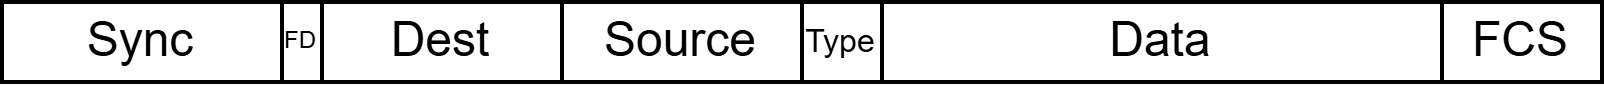
\includegraphics[width=0.5\linewidth]{images/eth.png}
    \caption{Ethernet frame}
\end{figure}
\noindent The frame includes the following key fields:
\begin{itemize}
    \item \textit{48-bit addresses}: these uniquely identify the source and destination devices.
    \item \textit{Type field}: this is a multiplexing field, used to indicate the type of data encapsulated in the frame.
    \item \textit{Data field}: this contains the actual data being transmitted.
    \item \textit{Frame check sequence}: a cyclic redundancy check used for error detection to ensure the integrity of the frame.
\end{itemize}

\paragraph*{MAC address}
The MAC address is crucial for filtering and routing Ethernet frames. 
The first 3 bytes of the MAC address identify the manufacturer of the network interface card, while the last 3 bytes are unique to each interface. 
An all-ones address is used for broadcast communication, ensuring the message reaches all devices on the network.

\paragraph*{CSMA/CD}
Ethernet networks originally used CSMA/CD as a method for managing access to the shared communication medium. 
In CSMA/CD, devices listen to the bus before transmitting to check if it is free. 
If the bus is clear, they proceed with transmission.
If a collision occurs, all transmissions are aborted, and devices wait a random amount of time before attempting to retransmit. 
This collision detection process ensures that communication is efficient, although it can introduce delays.

\paragraph*{Industry 4.0 ethernet}
In the context of Industry 4.0, Ethernet has been adapted for various use cases with different time-critical requirements. 
Ethernet in Industry 4.0 is classified into three classes based on the Maximum Cycle Time, which is a measure of the maximum time it takes to complete a cycle of communication:
\begin{itemize}
    \item \textit{Class A}: suitable for less time-sensitive industrial applications.
    \item \textit{Class B}: designed for applications that require faster communication.
    \item \textit{Class C}: this class supports the most demanding applications where extremely low-latency communication is essential.
\end{itemize}

\paragraph*{Hub and switches}
Ethernet networks traditionally used hubs, where all devices connected to the hub shared the same bandwidth, leading to potential collisions. 
In a hub-based setup, each device listens to the shared medium and can transmit only when it senses that the bus is free.

Fully switched LANs use network switches, which effectively eliminate collisions by providing a dedicated path between devices. 
In a switched Ethernet network, each device communicates directly with the switch, and each transmission is isolated, meaning that multiple devices can transmit simultaneously without interference. 
This removes the need for CSMA/CD, as there are no shared communication channels to compete for.

\subsection{Wireless}
The evolution of wireless networks has been largely driven by the rapid development of smart objects, which are interconnected devices capable of communicating over networks. 
These smart objects, including everything from sensors to consumer electronics, have become a central part of modern communication infrastructures, especially with the rise of the IoT.
Some possible wireless technologies are: 
\begin{itemize}
    \item \textit{Mobile radio networks}: evolving Radio Access Networks and Core Networks to meet growing data demands.
    \item \textit{Cellular IoT operators}: focused on low-power, wide-area connectivity for IoT devices.
    \item \textit{Low power long range technology}: enables long-distance communication with minimal power consumption, ideal for remote IoT applications.
    \item \textit{Capillary multi-hop networks}: distributed communication for short/medium-range with backhauling, extending coverage over multiple hops.
\end{itemize}